%% !TEX program = xelatex
%% -----------------------------------------------------------------
%% This file uses UTF-8 encoding
%%
%% For compilation use following command:
%% latexmk -xelatex -pvc -bibtex thesis
%%
%% -----------------------------------------------------------------
%%                                     _     _
%%      _ __  _ __ ___  __ _ _ __ ___ | |__ | | ___
%%     | '_ \| '__/ _ \/ _` | '_ ` _ \| '_ \| |/ _ \
%%     | |_) | | |  __/ (_| | | | | | | |_) | |  __/
%%     | .__/|_|  \___|\__,_|_| |_| |_|_.__/|_|\___|
%%     |_|
%%
%% -----------------------------------------------------------------

\documentclass{tukethesis}

\setdefaultlanguage{slovak}
\setotherlanguage{english}
%% For thesis written in English just swap the main and other languages:
% \setdefaultlanguage{english}
% \setotherlanguage{slovak}

% Additional packages


\addbibresource{bibliography.bib}   % Location of file with bibliography resources
\input{acronyms}                    % Load acronyms
%% Document Metadata

%% The location of your Assignment Statement (scanned as image)
% \thesisspec{figures/thesisspec.png}

%% Uncomment the following line for the final version without colored links
% \def\printable{}

\title {Kryptografia na báze eliptických kriviek}{Kryptografia na báze eliptických kriviek}
%\thesis{Master thesis}{Diplomová práca}  % typ prace

\author{Vladyslav}{Holovko}
\supervisor{prof. Ing. Miloš Drutarovský, CSc.}  % veduci prace
% \consultant{Leslie Lamport}  % konzultant
% \college{University of Žilina}{Žilinská univerzita}  % univerzita
% \faculty{Faculty of Electrical Engineering and informatics}{Fakulta elektrotechniky a informatiky}  % fakulta
% \department{Department of Computers and Informatics}{Katedra počítačov a informatiky}  % katedra
% \departmentacr{DCI}{KPI}  % skratka katedry
\submissiondate{13}{5}{2024}
% \fieldofstudy{Informatika}
% \studyprogramme{Informatika}
% \city{Košice}  % mesto

\keywords{%
  % english
  \LaTeX, programming, typesetting
}{%
  % slovak
  \LaTeX, programovanie, sadzba textu
}

\declaration{Vyhlasujem, že som záverečnú prácu vypracoval(a) samostatne s~použitím uvedenej odbornej literatúry.}

\abstract{%
  % english
  Abstract in English.
}{%
  % slovak
  Abstrakt v slovenčine.
}

\acknowledgment{%
Na tomto mieste by som rád poďakoval svojmu vedúcemu práce za jeho čas a odborné vedenie počas riešenia mojej záverečnej práce.
Rovnako by som sa rád poďakoval svojim rodičom a priateľom za ich podporu a povzbudzovanie počas celého môjho štúdia.
}
                    % Load thesis metadata
\usepackage{pgfplots} 
\usepackage{amsmath}  
\usepackage{pgfplots}
% Disable color links in the final version (define \printable in metadata.tex)
\ifdefined\printable
   \hypersetup{hidelinks}
\fi

%% -----------------------------------------------------------------
%%          _                                       _
%%       __| | ___   ___ _   _ _ __ ___   ___ _ __ | |_
%%      / _` |/ _ \ / __| | | | '_ ` _ \ / _ \ '_ \| __|
%%     | (_| | (_) | (__| |_| | | | | | |  __/ | | | |_
%%      \__,_|\___/ \___|\__,_|_| |_| |_|\___|_| |_|\__|
%%
%% -----------------------------------------------------------------

\begin{document}

%% Title page, abstract, declaration etc.:
\frontmatter{}

%% List of thesis chapters in required order
% \include{chapters/00-preface}
% !TEX root = ../thesis.tex

\chapter{Úvod}\label{ch:introduction}


Úvod práce stručne opisuje stanovený problém, kontext problému a motiváciu pre riešenie problému. Z úvodu by malo byť jasné, že stanovený problém doposiaľ nie je vyriešený a má zmysel ho riešiť.

V úvode neuvádzajte štruktúru práce, t.j. o čom je ktorá kapitola. Rozsah úvodu je minimálne 2 celé strany (vrátane formulácie úlohy).

\section*{Formulácia úlohy}

V rámci úvodu tiež vysvetlite vaše chápanie úlohy, ktorú budete riešiť. Prvú verziu tejto časti by ste mali napísať čo najskôr, aby ste sa uistili, že rozumiete, čo je cieľom vašej práce, a prekonzultovali ju so školiteľom. Neskôr v priebehu práce na projekte ju môžete spresňovať a dopĺňať.

%% Include other chapters here, e.g.:
% \include{chapters/02-current-state}
% \include{chapters/03-existing-solutions}
% ...
% !TEX root = ../thesis.tex

\chapter{Vyhodnotenie}\label{ch:evaluation}
\section{Matematické pozadie}\label{ch:problem}
\subsection{Konečné polia}

Prejdime k základom matematiky, konkrétne k definícii základov konečných polí a k tomu, čím sa líšia od skupín.
najprv prejsť k základom konečných polí, polí vo všeobecnosti a
skupín.
Skupina je množina prvkov spolu s operátorom, ktorý kombinuje ľubovoľné dva prvky skupiny a vytvára tretí prvok. Tento operátor musí spĺňať štyri podmienky, známe aj ako axiómy grupy:

\begin{itemize}
	\item Uzavretosť: všetky vytvorené prvky sú tiež v skupine.
	\item Asociatívnosť: ∀a, b, c: (a ◦ b) ◦ c = a ◦ (b ◦ c), kde ◦ je použitý operátor.
	\item  Identita: existuje prvok Id taký, že ∀a: (a ◦ Id = a).
	\item Invertibilita: každý prvok a v skupine má inverziu, takže
	a ◦ a-1 = Id.
\end{itemize}

Ak okrem toho spĺňa rovnicu komutatívnosti a◦b = b◦a,
nazýva sa abelická grupa. V prípade kombinácie množiny celých čísel
s operátorom +, ◦ = +, Id = 0 a a-1 = -a, pretože a + b = b + a,
je to tiež abelovská grupa.

Konečné pole Fp, nazývané aj Galoisovo pole, používané v eliptickej krivke
je pole s konečným počtom prvkov. Rád p
poľa je počet prvkov v ňom. Pole je abelovská grupa s
sčítaním a ďalším operátorom, a to násobením. Sčítanie spĺňa
všetky podmienky z abelických skupín. Násobenie je uzavreté, asociatívne
a komutatívna rovnako ako sčítanie. Okrem toho má
vlastný neutrálny prvok 1, kde 1 - a = a - 1 = a pre nejaký prvok
a. Každý prvok okrem 0 má inverzný prvok aj pre násobenie,
a - a-1 = a-1 - a = 1. Napokon, násobenie je distribučné s
vzhľadom na sčítanie, t. j. ∀a, b, c: (a - (b + c) = a - b + a - c).

\subsection{Elliptic curves}

Nech \( F \) je pole a \( E \) je krivka definovaná nad týmto poľom \( F \). Množina riešení \( E(F) \) pre nasledujúcu všeobecnú rovnicu je:

\[
y^2 = x^3 + ax^2 + bx + c
\]

kde \( a, b, c \in F \).

Pre nás sú zaujímavejšie Montgomeryho krivky, pretože sa používajú v NaCl knižnici. Všeobecne platí, že Montgomeryho krivky vyžadujú menej kódu a sú odolnejšie voči časovým útokom v porovnaní s bežnými eliptickými krivkami \cite{OKS00}. 

Montgomeryho krivka \( E \) má tvar:

\[
E(F_p) = \{\infty\} \cup \{(x, y) \in F_p : B y^2 = x^3 + Ax^2 + x \}
\]

kde \( \infty \) predstavuje "bod v nekonečne", ktorý slúži ako identita, a \( A \) je veľké celé číslo, pričom platí \( A^2 - 4 \neq \text{štvorec modulo} \, p \). Táto krivka by nemala mať žiadne vrcholy (ostrý bod) ani vlastné priesečníky, čo je dôležité, pretože potrebujeme krivku, ktorá je diferencovateľná (krivka s vrcholmi nemá jedinečnú deriváciu v bode vrcholu).

Následne môžeme definovať operáciu sčítania na tejto krivke, aby sme mohli implementovať kryptografické operácie. Spolu s bodom nekonečna tvoria body na krivke abelickú skupinu.

	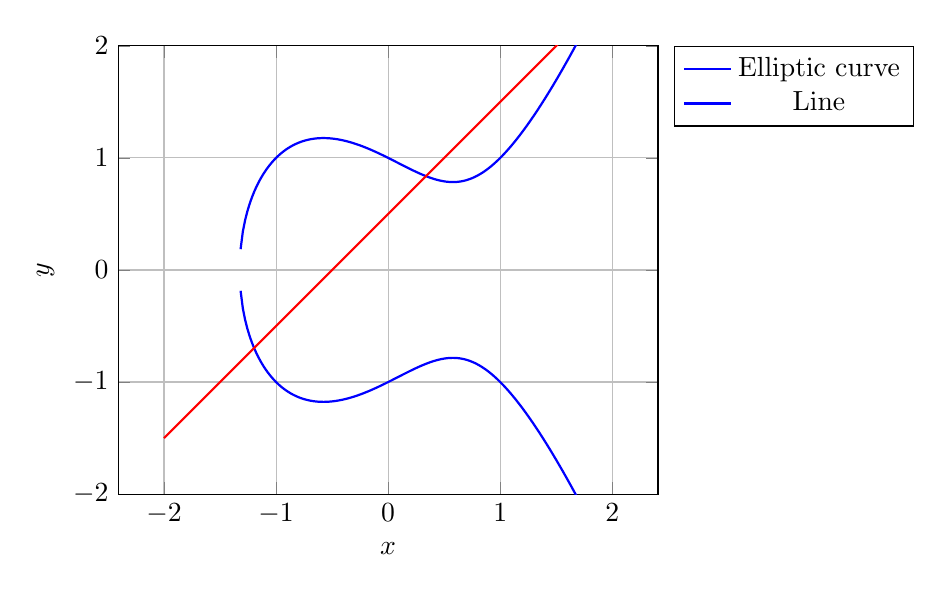
\begin{tikzpicture}
		\begin{axis}[
			axis equal,
			xlabel={$x$},
			ylabel={$y$},
			domain=-2:2,
			samples=100,
			grid=major,
			xmin=-2, xmax=2, ymin=-2, ymax=2,
			legend pos=outer north east
			]
			
			% Normalized elliptic curve y^2 = x^3 - x + 1
			\addplot [
			blue,
			thick,
			samples=200,
			domain=-2:2,
			] ({x}, {sqrt(x^3 - x + 1)});
			
			\addplot [
			blue,
			thick,
			samples=200,
			domain=-2:2,
			] ({x}, {-sqrt(x^3 - x + 1)});
			
			% Line intersecting the curve
			\addplot [
			red,
			thick,
			domain=-2:2,
			] {x + 0.5};
			
			\legend{Elliptic curve, Line}
			
		\end{axis}
	\end{tikzpicture}


Začneme s binárnym operátorom \( + \), ktorý môžeme najjednoduchšie opísať slovami: zoberte rôzne body \( A \) a \( B \), ktoré chceme sčítať, a nakreslite priamku cez tieto body. Existuje presne jeden ďalší bod priesečníka na krivke. Vypočítajte, kde sa nachádza tento tretí bod, a potom ho odrazte o os \( x \). 

„Dvojnásobenie“ bodu sa vykonáva tak, že vezmeme dotyčnicu v bode \( A \), potom vypočítame druhý bod priesečníka a vezmeme negáciu tohto bodu. Ak je priamka paralelná k osi \( y \), vezmeme identitný prvok \( \infty \). Na základe toho môžeme definovať operáciu \( + \) nasledovne: \\ \\
1. \( \infty + \infty = \infty \) \\
2. \( \infty + (x, y) = (x, y) + \infty = (x, y) \) \\
3. \( (x, y) + (x, -y) = \infty \) \\
4. Ak \( y \neq 0 \), potom \( (x, y) + (x, y) = (x'', y'') \), kde \( x'' = \lambda - A - 2x = \frac{(x^2 - 1)^2}{4y^2} \) a \( y'' = \lambda(x - x'') - y \). \( \lambda \) označuje prvú deriváciu \( E \), pričom \( \lambda = \frac{3x^2 + 2Ax + 1}{2y} \). (Dvojnásobenie bodu) \\
5. Ak \( x \neq x' \), potom \( (x, y) + (x', y') = (x'', y'') \), kde \( x'' = \Delta^2 - A - x - x' \) a \( y'' = \Delta(x - x'') - y \). Tu je \( \Delta \) definované ako \( \Delta = \frac{y' - y}{x' - x} \), inými slovami, je to sklon funkcie medzi bodmi \( (x, y) \) a \( (x', y') \). (Sčítanie) \\

Sčítanie identitného prvku a iného prvku \( X \) vedie k \( X \), ako je vidieť v (1) a (2). Sčítanie bodu a jeho negácie tiež vedie k identitnému prvku (3). V (4) sa dvojnásobenie bodu vykonáva najskôr výpočtom prvej derivácie, potom vypočítaním dotyčnice a vzatím negácie \( y \). V prípade, že \( y = 0 \), platí \( (x, 0) + (x, 0) = \infty \). (5) definuje „normálne“ sčítanie, kde vezmeme sklon medzi dvoma priamkami \( \Delta \) a vypočítame tretí bod \( x'' \). Ak \( x = x'' \), potom bude platiť (4). 


Sčítanie identitného prvku a iného prvku \( X \) vedie k \( X \), ako je vidieť v (1) a (2). Sčítanie bodu a jeho negácie tiež vedie k identitnému prvku (3). V (4) sa dvojnásobenie bodu vykonáva najskôr výpočtom prvej derivácie, potom vypočítaním dotyčnice a vzatím negácie \( y \). V prípade, že \( y = 0 \), platí \( (x, 0) + (x, 0) = \infty \). (5) definuje „normálne“ sčítanie, kde vezmeme sklon medzi dvoma priamkami \( \Delta \) a vypočítame tretí bod \( x'' \). Ak \( x = x'' \), potom bude platiť (4). Na obrázku 1b môžeme vidieť dvojnásobenie bodu, zatiaľ čo na obrázku 1a môžeme vidieť sčítanie.

\subsection{Eliptické krivky nad \( F_p \)}

Uvedená aritmetika je pomalá a nie je vhodná na kryptografické účely, pretože potrebujeme nekonečný počet bodov. Je potrebné niečo rýchle a presné, aby sme získali konečnú skupinu pre úlohu diskrétnych logaritmov. Toho dosiahneme kombináciou eliptických kriviek a predtým spomenutých konečných polí: eliptické krivky nad \( F_p \). Táto eliptická krivka \( E(F_p) \) obsahuje všetky body \((x, y)\), ktoré spĺňajú rovnicu eliptickej krivky modulo \( p \): \( y^2 \mod p = x^3 + Ax^2 + x \mod p \). 

\begin{figure}[h]
	\centering
	\begin{tikzpicture}
		\begin{axis}[
			width=15cm, % Ширина графика
			height=15cm, % Высота графика
			axis lines=middle,
			xlabel={$x$},
			ylabel={$y$},
			xlim={-7.5:7.5}, % Ограничения по оси x
			ylim={-7.5:7.5}, % Ограничения по оси y
			xtick={-7, -5, ..., 7},
			ytick={-7, -5, ..., 7},
			grid=both,
			minor tick num=1,
			major grid style={line width=.5pt,draw=gray!50},
			minor grid style={line width=.5pt,draw=gray!20}
			]
			% Здесь мы рисуем точки
			\addplot[only marks, mark=*] coordinates {
				(1, 2)
				(3, 5)
				(4, 3)
				(5, 6)
				(6, 7)
				(7, 8)
				(0, 0)
				(2, 2)
				(4, 4)
				(6, 6)
				(3, 1)
				(5, 2)
			};
		\end{axis}
	\end{tikzpicture}
	\caption{Graf}
	\label{fig:elliptic_curve}
\end{figure}
\include{chapters/09-summary}

%% Bibliography, glossary, acronyms
\backmatter{}


%% -----------------------------------------------------------------
%%                                       _ _
%%       __ _ _ __  _ __   ___ _ __   __| (_) ___ ___  ___
%%      / _` | '_ \| '_ \ / _ \ '_ \ / _` | |/ __/ _ \/ __|
%%     | (_| | |_) | |_) |  __/ | | | (_| | | (_|  __/\__ \
%%      \__,_| .__/| .__/ \___|_| |_|\__,_|_|\___\___||___/
%%           |_|   |_|
%% -----------------------------------------------------------------

% !TEX root = ../thesis.tex

\chapter*{\appendixlistname}
\addcontentsline{toc}{chapter}{\appendixlistname}

\begin{description}

   \item[\autoref{app:user.manual}] \nameref{app:user.manual}
   \item[\autoref{app:system.manual}] \nameref{app:system.manual}
   \item[\autoref{app:structure}] \nameref{app:structure}
   \item[\appendixname{} D] CD médium -- záverečná práca v~elektronickej podobe,
   \item[\appendixname{} E] Repozitár výsledného projektu je dostupný na adrese\\ \url{https://git.kpi.fei.tuke.sk/kpi/karel-the-robot}
\end{description}

\appendix
\renewcommand\chaptername{\appendixname}
% !TEX root = ../thesis.tex

\chapter{Používateľská príručka}\label{app:user.manual}


\include{appendixes/system.manual}
% !TEX root = ../thesis.tex

\chapter{Štruktúra záverečnej práce}\label{app:structure}

Na písanie záverečných prác je možné použiť viacero štruktúr. Pre vytvorenie tejto práce sme použili dve z~nich:

\begin{enumerate}
    \item hlavná štruktúra práce bola vytvorená podľa štruktúry uvedenej v~článku \cite{Beel2010}
    \item pre vytvorene abstraktu bola použitá štruktúra \cite{WikipediaImrad}, ktorá môže byť použitá na napísanie celej práce
\end{enumerate}

Krátky význam jednotlivých kapitol bude uvedený v~nasledujúcom texte. Ďalšie užitočné informácie nájsdete v~\emph{Pokynoch pre vypracovanie záverečných prác}\footnote{\url{https://theses.kpi.fei.tuke.sk/instructions}}.


\section*{Abstrakt}

% https://www.scribbr.com/dissertation/abstract/

Abstrakt by mal byť dlhý 100 až 300 slov. Pre jeho organizáciu môžete použiť štruktúru \emph{IMRaD}, čo je skratka pre:

\begin{itemize}
    \item \textbf{Introduction} - jasne predstavte zámer svojej práce, použite prítomný alebo minulý čas
    \item \textbf{Methods} - uveďte použité výskumné metódy, použite minulý čas
    \item \textbf{Results} - zhrňte hlavné dosiahnuté výsledky, použite prítomný alebo minulý čas
    \item \textbf{Discussion} - na záver zhrňte hlavné závery vyplývajúce z~vašej práce, použite prítomný čas
\end{itemize}

Na základe uvedenej štruktúry môžete abstrakt napísať tak, že každý bod napíšete v~jednej, ale maximálne v~dvoch vetách. Určite však do abstraktu neprepisujte obsah práce! Snažte sa, aby ste abstrakt spolu s~bibliografickou citáciou mali na jednej strane!


\section*{Predhovor}

Predhovor ponúka neformálny priestor na vlastné vyjadrenie autora. Môže obsahovať informácie o~tom, čo sa autor pri písaní práce naučil, o~vlastnej motivácii k~výberu témy, o~prekonaných výzvach počas písania práce, a pod. Píše sa v~prvej osobe jednotného čísla a rozsah by nemal presiahnuť 2 strany.

Táto kapitola nie je povinná!


\section*{Úvod}

Úvod práce stručne opisuje stanovený problém, kontext problému a motiváciu pre jeho riešenie. Z~úvodu by malo byť jasné, že stanovený problém má zmysel riešiť.

V~úvode neuvádzajte štruktúru práce! Rozsah tejto kapitoly by mal byť minimálne 2 strany.

Súčasťou úvodu je aj \emph{formulácia úlohy}.
Vo formulácii úlohy uveďte jasne a vecne ciele práce. Čím budú ciele konkrétnejšie, tým bude jasnejšie, aký problém riešite a ako ho chcete riešiť.
Formuláciu úlohy vytvorte po dostatočnom naštudovaní problematiky a vytvorení analytickej časti.

\section*{Analytická časť}

Analytická časť záverečnej práce analyzuje existujúce podobné prístupy k~riešeniu stanoveného problému. Autor práce musí uviesť v~tejto časti existujúce prístupy a riešenia, pričom musí zaujať stanovisko k~týmto prístupom a riešeniam a opísať ich výhody a nedostatky. Prevažne v~tejto časti autor používa odkazy na použité zdroje. Autor v~analýze nepreberá odseky z~cudzích prác ale uvádza prevažne vlastné postoje podložené odkazmi na literatúru. Analytická časť práce by teda nemala byť len povrchným prepisom základných informácií z~Wikipédie alebo zo stránok opisovaných nástrojov. Je potrebné aby bola analýza podporená aj experimentmi ak to umožňuje téma práce (napr. vyskúšam softvér). Vďaka popisu existujúcich riešení autor pochopí problematiku, viac sa nad riešeniami zamyslí, usporiada si ich, zistí ich kladné a záporné vlastnosti, z~čoho potom postupne vyplynie návrh vlastného riešenia v~syntetickej časti. Analytická časť tvorí zvyčajne ¼ jadra práce.

Analytickú časť je vhodné rozdeliť na niekoľko kapitol, ktoré budú venované rôznym analyzovaným témam. Názvy kapitol majú zodpovedať tomu, čo je v~kapitole opisované. Napríklad, ak v~práci analyzujete súčasný stav v~oblasti medzigalaktických letov, namiesto všeobecného názvu \enquote{Analýza súčasného stavu} by mal byť použitý názov analyzovanej témy -- \enquote{Medzigalaktické lety}.

Mali by ste v práci mať minimálne kapitoly opisujúce
\begin{itemize}
  \item doménu (oblasť) riešeného problému a jej súčasný stav,
  \item súvisiace práce a existujúce riešenia.
\end{itemize}

Je veľmi pravdepodobné, že sa daný problém pokúšal vyriešiť už aj niekto iný. Alebo existujú riešenia podobné tomu, ktoré potrebujete vyriešiť vy. V~tejto časti práce teda popíšete, aké riešenia už existujú a aké sú ich výhody a nevýhody. Týmto spôsobom preukážete, že ste si naštudovali tému a vyskúšali rôzne riešenia, a môžete sa inšpirovať už existujúcimi riešeniami.


\section*{Ciele záverečnej práce}

Vychádzajúc z analýzy problému a existujúcich riešení by ste mali byť schopní stanoviť konkrétne implementačné ciele vašej práce. Tie môžete uviesť v samostatnej kapitole, napríklad vo forme zoznamu alebo odrážok. Rozhodne tu neprepisujte zadávací list, ale jasne a stručne uveďte, svoje čiastkové ciele. Neskôr ich budete vedieť v~kapitole \emph{Vyhodnotenie} vyhodnotiť aj s~odôvodnením, či sa vám uvedené ciele splniť podarilo alebo nie.

\section*{Syntetická časť}

Syntetická časť opisuje metódy použité na syntézu riešenia a opisuje syntézu samotného riešenia (zvyčajne je to návrh/implementácia softvérového resp. hardvérového riešenia), pričom sa opiera o závery analytickej časti práce. Začína od toho, ako sa bude riešenie používať: najdôležitejšie scenáre používania a používateľské rozhranie, ktoré bude tieto scenáre efektívne podporovať. Až potom je na rade vnútorná architektúra alebo použité technológie. Syntetická časť tvorí zvyčajne ½ jadra práce.

Syntetickú časť práce vhodne rozdeľte do kapitol a pomenujte ich podľa toho, čomu sú venované. Podľa obsahu práce môže táto časť obsahovať kapitoly opisujúce, napríklad:

\begin{itemize}
  \item použitú metodológiu -- metodológia experimentu alebo spôsob riešenia úlohy,
  \item návrh riešenia -- celkový opis riešenia a jeho zdôvodnenie,
  \item implementáciu -- najpodstatnejšie implementačné rozhodnutia a ich zdôvodnenie.
\end{itemize}


\section*{Vyhodnotenie}

Vyhodnocovacia časť je kľúčovou časťou záverečnej práce. Tato časť obsahuje vyhodnotenie navrhnutého (vytvoreného) riešenia. Uprednostňované je objektívne vyhodnotenie výsledkov práce, ktoré sa opiera o meranie a štatistické metódy, prípadne matematické dôkazy. V prípade nameraných hodnôt musí autor opísať metódu merania, priebeh merania, výsledky a interpretáciu výsledkov v kontexte riešeného problému a stanovených cieľov. Na základe vyhodnotenia riešenia autor opíše prínosy svojej práce. Vyhodnocovacia časť tvorí zvyčajne ¼ jadra práce. 

Okrem iného môže byť súčasťou vyhodnotenia:
\begin{itemize}
  \item zhrnutie dosiahnutých výsledkov,
  \item interpretácia výsledkov,
  \item objektívne overenie dosiahnutia cieľov práce
\end{itemize}


\section*{Záver}

Záver práce obsahuje zhrnutie výsledkov práce s jasným opisom prínosov a pôvodných (vlastných) výsledkov autora a vyhodnotenie splnenia stanovených cieľov. Je to stručné zhrnutie informácií uvedených v záverečnej práci. Záver by nemal obsahovať nové informácie.

V závere by mal tiež autor poukázať na prípadné otvorené otázky, ktoré sú nad rámec rozsahu práce a mal by odporučiť ďalšie aktivity na pokračovanie pri riešení problému. Rozsah záveru je minimálne 1 celá strana.


\section*{Prílohy}

Prílohy môžu obsahovať doplňujúce materiály, ktoré sú dôležité pre pochopenie práce, ale nie sú nevyhnutné pre čitateľa, aby mohol pochopiť hlavný obsah práce. Prílohy majú obsahovať aj príručku pre používateľa a systémovú príručku pre nasadenie a pokračovanie vo vývoji.


\section*{Písanie v \LaTeX-u}

Odseky textu oddeľujte jednoducho prázdnym riadkom. To, že prvý odsek v kapitole nie je odsadený, je štandardný typografický postup a nie je potrebné ho meniť.

Časť textu môžeme \emph{mierne zvýrazniť} pomocou príkazu \verb|\emph{}|. Prípadne použiť \textbf{tučné písmo} príkazom \verb|\textbf{}|.

Na vytvorenie zoznamu sa používa prostredie \texttt{itemize}:

\begin{itemize}
  \item raz,
  \item dva,
  \item tri.
\end{itemize}

Zoznam môže byť aj číslovaný ak vymeníme \texttt{itemize} za \texttt{enumerate}:

\begin{enumerate}
  \item raz,
  \item dva,
  \item tri.
\end{enumerate}

\subsection*{Členenie textu}

Na definovanie kapitol a podkapitol sa používajú príkazy
\begin{itemize}
  \item \verb|\chapter{}|,
  \item \verb|\section{}|,
  \item \verb|\subsection{}|.
\end{itemize}

Hlbšie úrovne vnorenia sa neodporúča používať. Tak isto neodporúčame mnohonásobne vnorené zoznamy.

Ak za príkaz pridáte hviezdičku kapitola nebude číslovaná a ani sa nezobrazí v obsahu. Neodporúčame to však používať mimo príloh.

\subsection*{Obrázky}

Na vkladanie obrázkov sa používa prostredie \texttt{figure}:

\begin{figure}
  \centering
  \includegraphics[width=0.5\textwidth]{figures/tugboat}
  \caption{\LaTeX{} Friendly Zone \label{o:latex_friendly_zone}}
\end{figure}

Na samotné vloženie obrázka sa používa príkaz \verb|\includegraphics{}|. \LaTeX{} podporuje bežné formáty ako PNG a JPEG. Pre vektorovú grafiku je vhodné použiť formát PDF.

Každý obrázok by mal mať popis, ktorý je uvedený v~\emph{caption}. A čo je veľmi dôležité, na každý obrázok by mal byť odkaz v~texte. Na to použite príkazy \verb|\label{}| a \verb|\ref{}|. Prvý definuje názov, ktorým sa na obrázok odkazujete, druhý vytvorí odkaz na obrázok. Napríklad, obrázok \ref{o:latex_friendly_zone} zobrazuje prostredie priateľské pre používateľov \LaTeX-u.

\LaTeX{} má vstavené pravidlá pre umiestnenie obrázkov. Štandardne ich umiestni na vrch stránky, na ktorej sú definované, aby text nebol prerušený. Môžete však použiť voliteľné parametre, aby ste ovplyvnili umiestnenie obrázka. Napríklad \texttt{[!ht]} znamená, že obrázok sa má, ak je to možné, umiestniť presne tam, kde je definovaný, inak na vrchu stránky:

\begin{lstlisting}
\begin{figure}[!ht]
\end{lstlisting}

\subsection*{Tabuľky}

Tabuľky sa vkladajú do prostredí \texttt{table} a \texttt{tabular}

\begin{table}[!ht]
	\caption{Kódy krajín podľa štandardov ISO}\label{t:1}
	\smallskip
	\centering

	\begin{tabular}{llll}
		\toprule
		Názov krajiny & Alpha 2 & Alpha 3 & Numeric\\
		\midrule
		Afghanistan & AF & AFG & 004\\
		Alandské Ostrovy & AX & ALA & 248\\
		Albánsko & AL & ALB & 008\\
		Alžírsko & DZ & DZA & 012\\
		Americká Samoa & AS & ASM & 016\\
		Andorra & AD & AND & 020\\
		Angola & AO & AGO & 024\\
		\toprule
	\end{tabular}
\end{table}

Pre sadzbu profesionálne vyzerajúcich tabuliek odporúčame použiť balík \emph{booktabs}\footnote{\url{https://en.wikibooks.org/wiki/LaTeX/Tables\#Professional_tables}}.

\subsection*{Výpisy kódu}

Pre výpisy kódu sa používa prostredie \texttt{lstlisting}:

\begin{lstlisting}[language=C,caption={Program, ktorý pozdraví celý svet}, label={l:hello_world}]
#include <stdio.h>
int main() {
    /* Print Hello, World! */
    printf("Hello, World!\n");
    return 0;
}
\end{lstlisting}

Výpisy môžu mať voliteľný nadpis, ktorý sa zobrazí nad výpisom. Tak isto je možné im definovať \texttt{label}, na ktorý sa môžete odkazovať (viď výpis \ref{l:hello_world}).

Obsah výpisu môže byť tiež načítaný zo súboru pomocou príkazu:

\lstinputlisting[caption={Riešenie problému Schody},language=C]{listings/stairs.c}

\subsection*{Citácie}

Na citovanie literatúry sa používa balík \emph{biblatex}. Citácie sa vkladajú pomocou príkazu \verb|\cite{}|. Napríklad, \cite{Beel2010} je článok, ktorý popisuje štruktúru záverečnej práce.

Bibliografické záznamy sú definované v súbore \texttt{bibliography.bib}. Každý záznam má unikátny identifikátor, ktorý sa používa na citovanie. Napríklad, záznam \texttt{Beel2010} vyzerá nasledovne:


\begin{lstlisting}[breaklines=true, prebreak=\mbox{\textcolor{red}{$\hookleftarrow$}}]
@online{Beel2010,
  title  = {How to write a thesis (Bachelor, Master, or PhD) and which software tools to use},
  url    = {https://isg.beel.org/blog/2010/03/02/how-to-write-a-phd-thesis/},
  author = {Joeran Beel},
  year   = {2010},
  urldate = {2024-09-26}
}
\end{lstlisting}

Za znakom \texttt{@} je uvedený typ záznamu, v tomto prípade \texttt{online}. Iné typy záznamov môžu byť napríklad \texttt{article}, \texttt{book}, \texttt{inproceedings}, a pod. Každý záznam má povinné a nepovinné položky. Pre viac informácií o formáte záznamov v bibliografickom súbore odporúčame pozrieť stránku \emph{The 14 BibTeX entry types}\footnote{\url{https://www.bibtex.com/e/entry-types/}}.

Pri online zdrojoch nezabudnite uviesť dátum prístupu v položke \texttt{urldate}, keďže také zdroje sa môžu časom meniť.


%% -----------------------------------------------------------------
%%       ___ _   _ _ __ ___   _____   __
%%      / _ \ | | | '__/ _ \ / __\ \ / /
%%     |  __/ |_| | | | (_) | (__ \ V /
%%      \___|\__,_|_|  \___/ \___| \_/
%% -----------------------------------------------------------------

% Životopis autora
% \curriculumvitae\protect
%Táto časť\/ je nepovinná. Autor tu môže uviesť\/ svoje biografické
%údaje, údaje o~záujmoch, účasti na~projektoch, účasti na~súťažiach,
%získané ocenenia, zahraničné pobyty na~praxi, domácu prax, publikácie
%a~pod.

\end{document}
